% Uncomment this to make slides with overlays:
%\documentclass[slides]{beamer}

% Uncomment these (but comment the above \documentclass line) to make handouts:
\documentclass[handout]{beamer}

% Uncomment these to have more than one slide per page
\usepackage{pgfpages}
\pgfpagesuselayout{2 on 1}[border shrink=5mm]
\pgfpageslogicalpageoptions{1}{border code=\pgfusepath{stroke}}
\pgfpageslogicalpageoptions{2}{border code=\pgfusepath{stroke}}

\usepackage[]{graphicx, color, hyperref}

\mode<presentation>
{
	%\usetheme[secheader]{Boadilla}
	%\usecolortheme[rgb={.835, .102,.169}]{structure}  
	\usetheme[width= 0cm]{Goettingen}
	%\setbeamercovered{transparent}
}
\setbeamertemplate{navigation symbols}{}
\setbeamertemplate{footline}[frame number]

\definecolor{blue2}{rgb}{0.278,0.278,0.729} 
\newcommand{\blue}[1]{\textcolor{blue2}{#1}}
\newcommand{\white}[1]{\textcolor{white}{#1}}
\newcommand{\red}[1]{\textcolor{red}{#1}}
\newcommand{\xbar}{\overline{x}}
\newcommand{\ybar}{\overline{y}}
\newcommand{\phat}{\widehat{p}}
\newcommand{\prob}{\mbox{Pr}}
\newcommand{\E}{\mathbb{E}}
\newcommand{\Var}{\mbox{Var}}
\newcommand{\cp}{\oplus}
\newcommand{\cm}{\circleddash}

\title{Lecture 13: Confidence Intervals}
\author{Chapter 4.2}


\begin{document}
%------------------------------------------------------------------------------
\begin{frame}
\titlepage
\end{frame}
%------------------------------------------------------------------------------


%------------------------------------------------------------------------------
\begin{frame}[fragile]
\frametitle{Previously... Behavior of Point Estimates}
Say we draw a random sample of size $n=100$ from a large population that has true population mean $\mu=5$ and $\sigma=2$.

\vskip 0.5cm

\begin{center}
\begin{tabular}{ll}
Do this for the 1st time & We get, say, $\overline{x}=4.831$\\
Do this for the 2nd time & We get, say, $\overline{x}=5.104$\\
Do this for the 3rd time & We get, say, $\overline{x}=4.965$\\
\ldots & \\
Do this for the 1000th time & We get, say, $\overline{x}=4.957$
\end{tabular}
\end{center}

\vskip 0.5cm

The \blue{sampling distribution of $\xbar$} describes how these different instances $\xbar$ behave!

\end{frame}
%------------------------------------------------------------------------------



%-------------------------------------------------------------------------------
\begin{frame}
\frametitle{Previously... Sampling Distribution}
Each element in this histogram is one of 1000 instances of $\xbar$, where each $\xbar$ is computed from a sample of $n=100$ values.
\setkeys{Gin}{width=0.7\textwidth}
\begin{center}
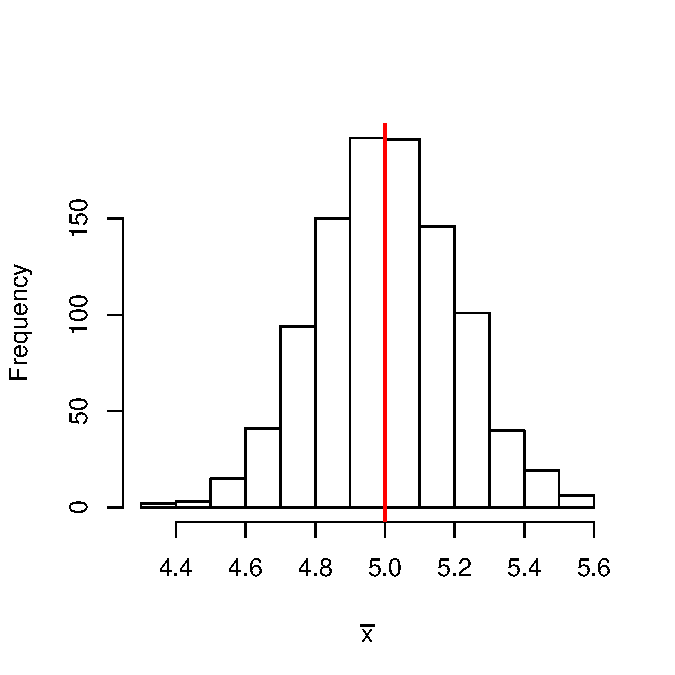
\includegraphics{figure/lec12-001}
\end{center}
\end{frame}
%-------------------------------------------------------------------------------





%------------------------------------------------------------------------------
\begin{frame}[fragile]
\frametitle{Previously... Sampling Distributions}

Intuitively: the \blue{sampling distribution} describes the (random) behavior of point estimates based on samples of fixed size $n$.  

\pause \vspace{0.5cm}
In the previous slide
\begin{itemize}
\pause \item \blue{center}: the mean of the sampling distribution is the true mean $\mu=5$.
\pause \item \blue{spread}: the standard deviation of the sampling distribution is called the \blue{standard error SE}.  It describes the error associated with the point estimate.  
\end{itemize}

\end{frame}
%------------------------------------------------------------------------------



%------------------------------------------------------------------------------
\begin{frame}[fragile]
\frametitle{Previously... Standard Error of the Sample Mean $\xbar$}

Given $n$ independent observations from a population with standard deviation $\sigma$, the \blue{standard error of the sample mean} is
\[
SE = \frac{\sigma}{\sqrt{n}}
\]

\pause A good way to ensure independence of observations is to draw a simple random sample that's less than 10\% of the population.  

\vspace{0.5cm}

\pause When
\begin{itemize}
\item the sample size is at least 30
\item the population distribution is \blue{not} strongly skewed
\end{itemize}
\pause we can use the point estimate of the standard deviation from the sample.  i.e. plug in $s$ in place of $\sigma$:
\[
SE = \frac{s}{\sqrt{n}}
\]

\end{frame}
%------------------------------------------------------------------------------





%------------------------------------------------------------------------------
\begin{frame}[fragile]
\frametitle{Concept:  Accuracy vs Precision}

\begin{itemize}
\pause \item \blue{accuracy} has to do with bias:  ``Does $\overline{x}$ on average hit $\mu$?''
\pause \item \blue{precision} has to to with error:  ``How reliable is $\overline{x}$?''
\end{itemize}

\vspace{5cm}

\end{frame}
%------------------------------------------------------------------------------





%------------------------------------------------------------------------------
\begin{frame}[fragile]
\frametitle{Goals for Today}

\begin{itemize}
\item Introduce confidence intervals
\item Give an informal description of the central limit theorem
\item Interpretation
\end{itemize}

\end{frame}
%------------------------------------------------------------------------------



%------------------------------------------------------------------------------
\begin{frame}[fragile]
\frametitle{Intuition of a Confidence Interval}

\blue{Our Goal}:  we want estimate a population parameter (e.g. $\mu$).

\blue{Analogy from book}: imagine the population parameter is a fish in a murky river.  We want to capture this fish.

\pause \vspace{0.25cm}

\begin{columns}
	\column{.45\textwidth} 
  Using just the point estimate:
  \column{.45\textwidth}
  Using a \blue{confidence interval}:
\end{columns}

\begin{center}
\includegraphics[height=4cm]{figure/spear.jpg}
\hspace{0.2cm}
\includegraphics[height=4cm]{figure/net.jpg}
\end{center}



\end{frame}
%------------------------------------------------------------------------------




%------------------------------------------------------------------------------
\begin{frame}[fragile]
\frametitle{Intuition of a Confidence Interval}

Recall that we had the following sampling distribution of 1000 instances of $\xbar$ where each $\xbar$ is based on $n=100$.  Keep in mind this was an unrealistic situation where we \blue{know} $\mu=5$ \& $\sigma=2$.  

\setkeys{Gin}{width=0.4\textwidth}
\begin{center}
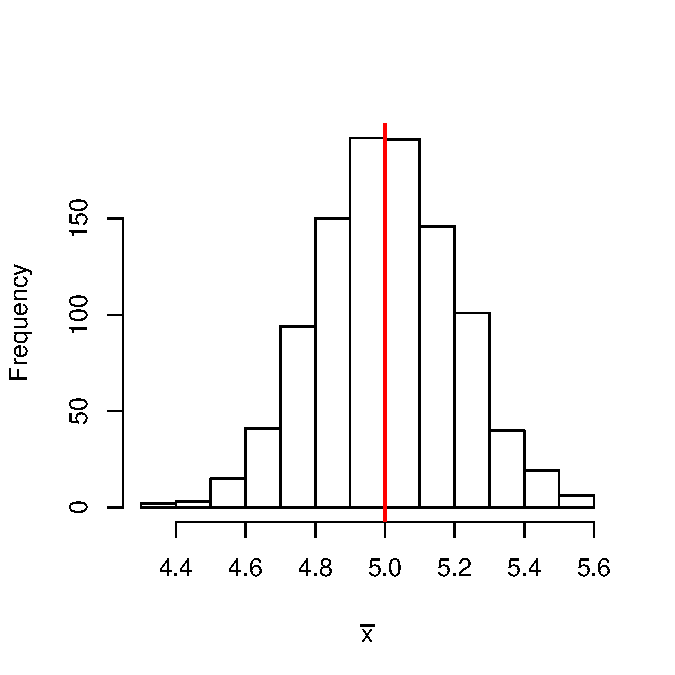
\includegraphics{figure/lec12-001}
\end{center}

We observe the sampling distribution
\begin{itemize}
\item is centered at $\mu$
\item has $SE = \frac{\sigma}{\sqrt n} = \frac{2}{\sqrt{100}} = 0.2$
\end{itemize}

\end{frame}
%------------------------------------------------------------------------------




%------------------------------------------------------------------------------
\begin{frame}[fragile]
\frametitle{Intuition of a Confidence Interval}
A plausible range of values for the population parameter is called a \blue{confidence interval (CI)}.  Since
\begin{itemize}
\pause \item the SE is the standard deviation associated with $\xbar$\\
 i.e. the SD of the sampling distribution
\pause \item roughly 95\% of the time $\xbar$ will be within 2 SE of the parameter $\mu$
\end{itemize}

\pause If the interval spreads out 2 SE from $\xbar$, we can be roughly
\blue{``95\% confident''} that we have captured the true parameter $\mu$.  
\end{frame}
%------------------------------------------------------------------------------




%------------------------------------------------------------------------------
\begin{frame}[fragile]
\frametitle{Intuition of a Confidence Interval}
So a \blue{rough} confidence interval is:

\begin{eqnarray*}
\xbar \pm  2 SE &=& \left[\xbar - 2 SE, \mbox{  }\xbar + 2 SE\right]\\
\xbar \pm 2 \frac{\sigma}{\sqrt{n}} &=& \left[\xbar - 2 \frac{\sigma}{\sqrt{n}}, \mbox{  }\xbar + 2 \frac{\sigma}{\sqrt{n}}\right]
\end{eqnarray*}

\pause But since we will typically not know $\sigma$, assuming the conditions hold we throw in $s$ in place of $\sigma$
\begin{eqnarray*}
\xbar \pm 2 \frac{s}{\sqrt{n}} &=& \left[\xbar - 2 \frac{s}{\sqrt{n}}, \mbox{  }\xbar + 2 \frac{s}{\sqrt{n}}\right]
\end{eqnarray*}



\end{frame}
%------------------------------------------------------------------------------



%-------------------------------------------------------------------------------
\begin{frame}
\frametitle{Central Limit Theorem}

\pause \blue{Central Limit Theorem} (informal description, more thorough treatment in Chapter 4.4):\\

\vspace{0.5cm}

\pause If a sample consists of at least 30 independent observations and the data are not
strongly skewed, then the distribution of the sample mean $\xbar$ is well approximated by
a \blue{normal model}.


\end{frame}
%-------------------------------------------------------------------------------



%-------------------------------------------------------------------------------
\begin{frame}
\frametitle{Confidence Intervals}

A 95\% confidence interval for the mean is more precise using $z^* = 1.96$, and not 2.  
\[
\left[\xbar - 1.96 SE, \mbox{  }\xbar + 1.96 SE\right] = 
\left[
\overline{x} - 1.96 \times\frac{s}{\sqrt n}, \mbox{  }
\overline{x} + 1.96 \times\frac{s}{\sqrt n}
\right]
\]


\pause A 99\% confidence interval for the mean
\[
\left[\xbar - 2.58 SE, \mbox{  }\xbar + 2.58 SE\right] = 
\left[
\overline{x} - 2.58 \times\frac{s}{\sqrt n}, \mbox{  }
\overline{x} + 2.58 \times\frac{s}{\sqrt n}
\right]
\]


\end{frame}
%-------------------------------------------------------------------------------





%-------------------------------------------------------------------------------
\begin{frame}
\frametitle{Conditions Needed}
Important conditions to help ensure the sampling distribution of $\xbar$ is nearly normal
and the estimate of $SE=\frac{s}{\sqrt n}$ is sufficiently accurate:
\begin{itemize}
\pause \item The sample observations are independent.
\pause \item The sample size is large: $n \geq 30$ is a good rule of thumb.
\pause \item The distribution of sample observations is not strongly skewed.
\end{itemize}

\pause Additionally, the larger the sample size, the more lenient we can be with the
sample's skew.

\end{frame}
%-------------------------------------------------------------------------------




%-------------------------------------------------------------------------------
\begin{frame}
\frametitle{Everyday Example:  Political Polls}
You look at a news article online and it says:
\begin{quotation}
\noindent We polled the electorate and found that 45\% of voters plan to vote for candidate $X$.  The margin of error for this poll is $\pm 3.4$ percentage points 19 times out of 20.  
\end{quotation}
\pause What does this mean?
\begin{itemize}
\pause \item ``19 times out of 20'' indicates 95\%
\pause \item The \blue{margin of error} of $\pm 3.4$\% indicates that 95\% C.I. is:
\[45 \pm 3.4 \% = [41.6, 48.4]\]
\end{itemize}
\textcolor{white}{Remember: the interpretation is not that there is a 95\% chance that $[41.6, 48.4]$ captures the true \%'age of people who will vote for candidate X.  Rather, that if we were to take 20 such polls, 19 of them would capture the true \%'age.}
\end{frame}
%-------------------------------------------------------------------------------




%-------------------------------------------------------------------------------
\begin{frame}
\frametitle{Crucial: How to Interpret a Confidence Interval}
The confidence interval has nothing to say about any particular calculated interval; it only pertains to the \blue{method} used to construct the interval:
\vskip 0.25cm
\begin{itemize}
\pause \item\blue{Wrong, yet common, interpretation}:  There is a 95\% chance that the C.I. captures the true population mean $\mu$
%--------------------
\pause \item\blue{Correct, interpretation}:  If we were to repeat this sampling procedure 100 times, we expect 95 (i.e. 95\%) of calculated C.I.'s to capture the true $\mu$
\end{itemize}
 
\end{frame}
%-------------------------------------------------------------------------------



%-------------------------------------------------------------------------------
\begin{frame}
\frametitle{Illustration:  How to Interpret a Confidence Interval}
At the outset of Chapter 4, there is an example data set of finish times (in minutes) from the 2012 Cherry Blossom 10 mile run, which had 16,924 participants.  In this case, we can compute the \blue{true} population mean $\mu=94.52$.

\vspace{0.5cm}

\pause Say we take 25 (random) samples of size $n=100$ (less than 10\% of 16,924), and each time we compute:
\begin{itemize}
\item $\xbar$
\item $s$
\item and hence the 95\% CI:  $\left[
\overline{x} - 1.96 \times\frac{s}{\sqrt n}, \mbox{  }
\overline{x} + 1.96 \times\frac{s}{\sqrt n}
\right]$
\end{itemize}
\pause We then observe
\end{frame}
%-------------------------------------------------------------------------------



%-------------------------------------------------------------------------------
\begin{frame}
\frametitle{How to Interpret a Confidence Interval}

\begin{center}
\includegraphics[width=8cm]{figure/CI.png}
\end{center}

\end{frame}
%-------------------------------------------------------------------------------



%-------------------------------------------------------------------------------
\begin{frame}
\frametitle{How to Interpret a Confidence Interval}
In this case, of the 25 confidence intervals we generated based on 25 samples of size $n=100$, one of them (in red) did not capture the true population mean $\mu$.

\vspace{0.5cm}

\pause As stated earlier, if we were to \blue{repeat this whole procedure} (collect sample of size $n=100$ and compute $\xbar$, $s$ and the 95\% CI), we expected 95 of them to capture the true population mean $\mu$.  

\end{frame}
%-------------------------------------------------------------------------------



%-------------------------------------------------------------------------------
\begin{frame}
\frametitle{Back to Political Polls}
You look at a news article online and it says:
\begin{quotation}
\noindent We polled the electorate and found that 45\% of voters plan to vote for candidate $X$.  The margin of error for this poll is $\pm 3.4$ percentage points 19 times out of 20.  
\end{quotation}
What does this mean?
\begin{itemize}
\item ``19 times out of 20'' indicates 95\%
\item The margin of error of $\pm 3.4$\% indicates that 95\% C.I. is:
\[45 \pm 3.4 \% = [41.6, 48.4]\]
\end{itemize}
\pause \blue{Intrepretation}: the interpretation is not that there is a 95\% chance that $[41.6, 48.4]$ captures the true \%'age of people who will vote for candidate X.  Rather, that if we were to take 20 such polls, 19 of them would capture the true \%'age.
\end{frame}
%-------------------------------------------------------------------------------


%%-------------------------------------------------------------------------------
%\begin{frame}
%\frametitle{Sidebar: Bayesian Credible Intervals}
%\blue{Sidebar}:  this wacky interpretation is an unfortunate limitation of the classical \blue{frequentist} paradigm of statistics.  
%
%\vspace{0.5cm}
%
%Under the \blue{Bayesian} paradigm of statistics, \blue{credible intervals} (Bayesian counterpart to confidence intervals) have the more intuitive interpretation.
%
%\vspace{0.5cm}
%
%So say we did a Bayesian analysis of the race data and found a 95\% credible interval of $(92.45, 98.77)$ minutes.  
%
%\vspace{0.5cm}
%
%We can \blue{now} say \textit{there is a 95\% chance/probability that $(92.45, 98.77)$ captures the true population mean $\mu$}.  No notion of ``if we were to repeat this 100 times, then 95 of...''
%
%\end{frame}
%%-------------------------------------------------------------------------------




%------------------------------------------------------------------------------
\begin{frame}[fragile]
\frametitle{Next Time}

Hypothesis Testing:  we can perform \blue{statistical tests} on population parameters such as $\mu$:

\begin{itemize}
\item Null and alternative hypotheses.
\item Testing hypotheses using confidence intervals.
\item Types of errors
\end{itemize}


\end{frame}
%------------------------------------------------------------------------------







\end{document}










